\section{Results}

For our experimental run with a linear SVM, we achieved $86.13 \%$ accuracy, with the precision, recall, and F1-scores for this model displayed in Table 1.1. Moreover, using the random forest method, we achieved $92.06 \%$ accuracy with the aforementioned metrics for it displayed in Table 1.1 as well. We compare this to the result found in the experiment done by Calleja and Fuentes who also performed PCA and then random forest, which received an accuracy of $91.64 \%$. The difference between our experiment and the experiment done by Calleja and Fuentes is that we include a fourth class of classification, the invalid category. Calleja and Fuentes use only three classes: elliptical, spiral, and irregular. Regardless of this difference, we found that our random forest classifier was able to distinguish invalid images as well while achieving a slightly higher accuracy. We found that the accuracy of our random forest run was higher than that of our linear SVM, thus corroborating our Hypothesis 2.

\begin{figure}[H]
    \centering
    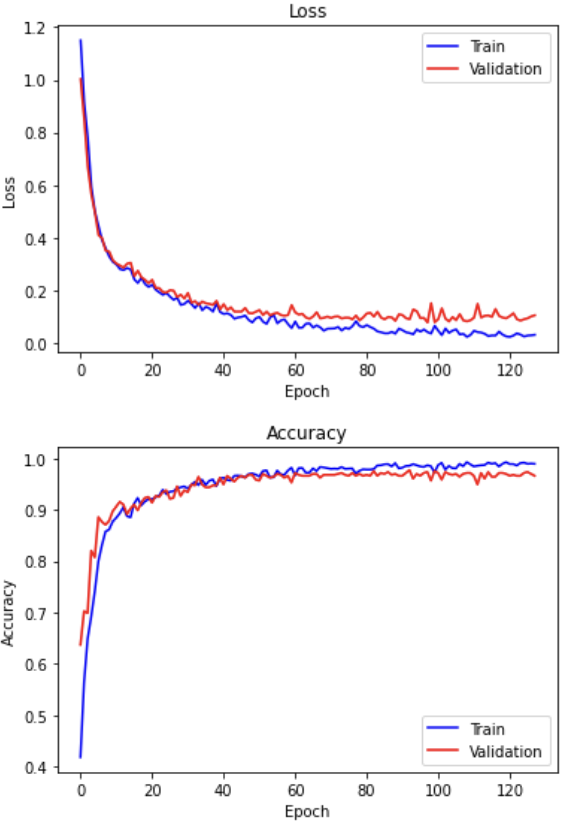
\includegraphics[width=0.5\textwidth]{Images/loss-accuracy-cnn.png}
    \caption{Loss and Accuracy plots generated for training and validation in Convolutional Neural Nets}
\end{figure}

The below Figure 1.9 shows the predictions of each image along with the actual class label. Table 1.1 displays the classification reports with precision, recall and F1-score for SVM classifier and Random Forest Classifier.

In Figure 1.7 and Figure 1.8, we see the ROC curve for the linear SVM and random forest classifiers, respectively. The ROC curves further evince that the random forest classifier achieves better performance than the linear SVM. We can see that in Figure 1.8, the true positive rate is very close to 1.0 while the false positive rate is very close to 0.0 for classes 2 and 3 compared to the curves in Figure 1.7 for classes 2 and 3 . We can also see that the curves for classes 0 and 1 are closer to the $(0,1)$ point of the curve in Figure 1.8 than in Figure 1.7.

\begin{table}
    \centering
    \caption{Classification Report of Linear SVM and Random Forest $P$-Precision, $R$ - Recall, F1 - F1 Score, WA - Weighted Average}
    
    \begin{tabular}{|c|c|c|c|c|c|c|}
    \hline
     & \multicolumn{3}{|c|}{Linear SVM} & \multicolumn{3}{|c|}{Random Forest} \\
    \hline
    Class & $\mathrm{P}$ & $\mathrm{R}$ & $\mathrm{F} 1$ & $\mathrm{P}$ & $\mathrm{R}$ & $\mathrm{F} 1$ \\
    \hline
    0 & 0.79 & 0.88 & 0.83 & 0.89 & 0.90 & 0.90 \\
    \hline
    1 & 0.86 & 0.81 & 0.84 & 0.92 & 0.85 & 0.89 \\
    \hline
    2 & 0.86 & 0.94 & 0.90 & 0.91 & 0.97 & 0.94 \\
    \hline
    3 & 0.97 & 0.80 & 0.88 & 0.96 & 0.97 & 0.96 \\
    \hline
    WA & 0.85 & 0.85 & $\mathbf{0 . 8 6}$ & 0.92 & 0.92 & $\mathbf{0 . 9 2}$ \\
    \hline
    \end{tabular}
    
\end{table}

\begin{figure}[H]
    \centering
    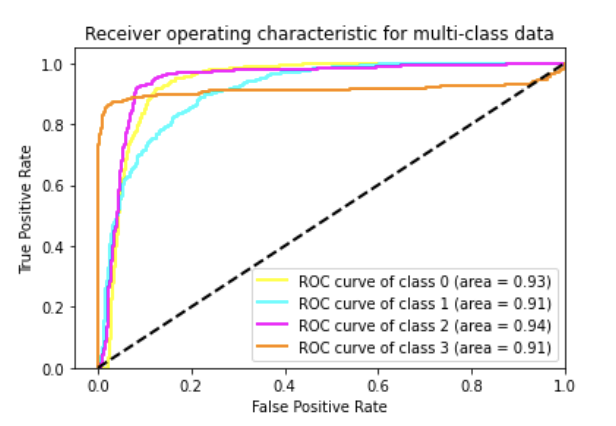
\includegraphics[width=0.5\textwidth]{Images/ROC-curve-SVM.png}
    \caption{ROC curve for the linear SVM}
\end{figure}

\begin{figure}[H]
    \centering
    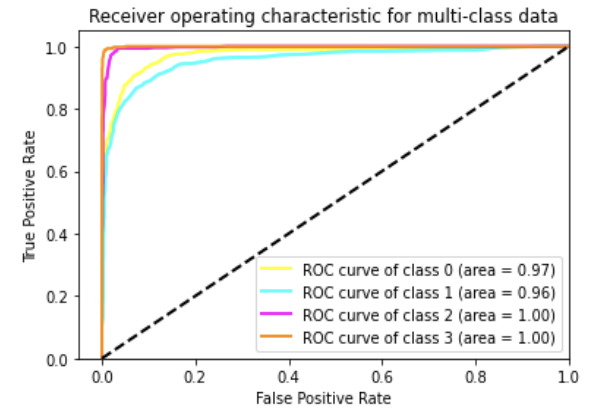
\includegraphics[width=0.5\textwidth]{Images/ROC-curve-rfc.png}
    \caption{ROC curve for the Random Forest Classifier}
\end{figure}

Our MLP model achieved classification accuracy of about $\mathbf{8 7 \%}$. We have shown the loss and accuracy plots for MLP in Figure 1.5. We also provide the classification report for our MLP model in Table 1.2. An interesting feature of our accuracy plot in Figure 1.5 is that the validation accuracy ends up being greater than the training accuracy as model training continues. However, it is still within the margin of error and is a weak indication of generalizable performance. In Figure 1.9, we show a sample of images with their actual and predicted class that resulted from the MLP model.

% Table 1.2: Classification Report of MLP and CNN

\begin{center}[H]
$\begin{array}{|c|c|c|c|c|c|c|}\hline&&\mathbf{MLP}&&&\mathbf{CNN}&\\\hline\text{Class}&\text{P}&\text{R}&\text{F1}&\text{P}&\text{R}&\text{F1}\\\hline0&0.80&0.85&0.82&0.95&0.98&0.96\\\hline1&0.86&0.88&0.82&0.97&0.93&0.95\\\hline2&0.93&0.89&0.91&0.98&0.97&0.97\\\hline3&0.88&0.96&0.92&0.97&0.98&0.98\\\hline\text{WA}&0.87&0.90&\textbf{0.87}&0.97&0.97&\textbf{0.97}\\\hline\end{array}$
\end{center} 

\begin{figure}[H]
    \centering
    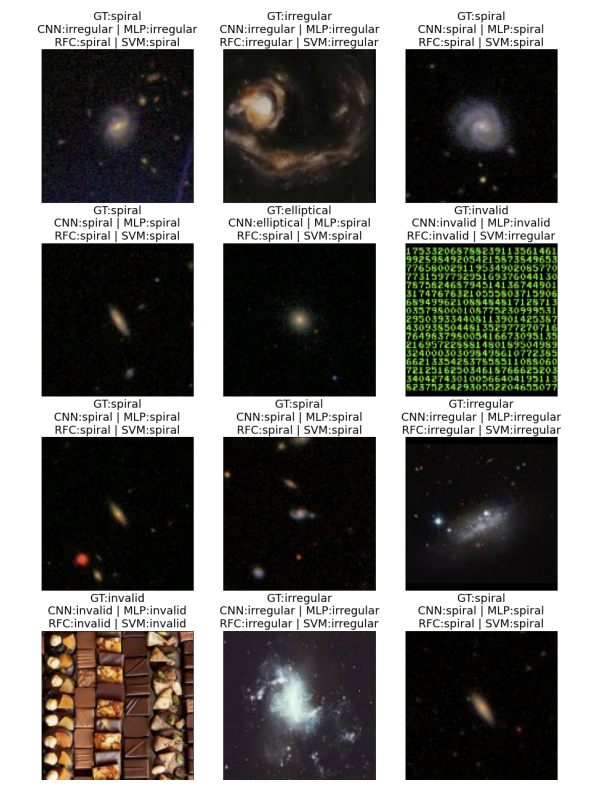
\includegraphics[width=0.5\textwidth]{Images/sample-images.png}
    \caption{Sample images with their actual and predicted class for RFC, SVM,MLP and CNN model}
\end{figure}

% GT:spiral\\
% CNN:irregular | MLP:irregu\\
% RFC:spiral | SVM:spiral

% GT:spiral\\
% CNN:spiral | MLP:spiral\\
% RFC:spiral | SVM:spiral

% GNN:ellipticlical | MLP:spiral

% \begin{center}
% \includegraphics[max width=\textwidth]{2024_05_01_50074901ee5ad42c853eg-6(1)}
% \end{center}

% CNN:invalid | MLP:invalic

% \begin{center}
% \includegraphics[max width=\textwidth]{2024_05_01_50074901ee5ad42c853eg-6}
% \end{center}

% GTi:rregular\\
% NN:\\
% Cirregular I MLP:irregula\\
% a RFC:irregular $\mid$ SVM:irregular

% CNN:spiral | MLP:spir

% RFC:spiral | SVM:spiral

% Figure 1.9 Sample images with their actual and predicted class for $R F C, S V M, M L P$ and CNN model

Our CNN model performed at an accuracy of $97 \%$. We have shown the loss and accuracy plots above in Figure 1.6. We also provide the classification report for our CNN model in Table 1.2. It is observed that as the hidden layers in the model are increased, the accuracy of the model increases. In Figure 1.9, we show a sample of images with their actual and predicted class that resulted from the CNN model.